\documentclass[]{article}

\usepackage{amsmath}
\usepackage{amsfonts}
\usepackage{amssymb}

\newtheorem{definition}{Definition}

\usepackage[]{algorithm2e}

\usepackage{booktabs}
\usepackage{rotating}

%%% for dags
\usepackage{tikz}
\usetikzlibrary{arrows}
\usetikzlibrary{fit,positioning, backgrounds}

%%% BibTex packages (url for website references)
\usepackage[english]{babel}
\usepackage[round]{natbib}

%opening
\title{Consensus clustering for Bayesian mixture models: Supplementary materials}
\author{Stephen Coleman, Paul DW Kirk\, and Chris Wallace}

\begin{document}

\maketitle

\begin{abstract}
Description of models used and analyses performed.
\end{abstract}

%\section{Algorithms} \label{sec:algorithms}

\section{Definitions}
\begin{definition}[Consensus matrix]
	Given $S$ clusterings for a dataset of $N$ items, $c_s=(c_{s1}, \ldots, c_{sN})$, the \emph{Consensus matrix} is a $N \times N$ matrix where the $(i, j )^{th}$ entry records the proportions of clusterings for which items $i$ and $j$ are allocated the same label. More formally, it is the matrix $\mathbb{C}$ such that
	\begin{align}
		\mathbb{C}(i, j) = \frac{1}{S} \sum_{s=1}^S \mathbf{I}(c_{si} = c_{sj})
	\end{align}
	where $\mathbb{I}(\cdot)$ is the indicator function taking a value of 1 is the argument is true and 0 otherwise.
\end{definition}

\begin{definition}[Posterior similarity matrix]
	A \emph{Consensus matrix} for which all the clusterings are generated from a converged Markov chain for some Bayesian clustering model. Sometimes abbreviated to \emph{PSM}.
\end{definition}

\section{The models} \label{sec:models}

\subsection{Individual dataset}
In the simulations (see section \ref{sec:simulations}) where individual datasets are modelled a \emph{Bayesian mixture model} is used. We write the basic mixture model for independent items $X=(x_1, \ldots, x_N)$ as 
\begin{align}
	x_i \sim \sum_{k=1}^K\pi_k f(x_i | \theta_k) \hspace{1cm} \textrm{independently for $i = 1,\ldots,N$}
\end{align}
where $f(\cdot| \theta)$ is some family of densities parametrised by $\theta$. A common choice is the Gaussian density function, with $\theta=(\mu, \sigma^2)$. This is model used in the simulation study. $K$, the number of subgroups in the population, $\{\theta_k\}_{k=1}^K$, the component parameters, and $\pi=(\pi_1, \ldots, \pi_K)$, the component weights are the objects to be inferred. In the context of \emph{clustering}, such a model arises due to the belief that the population from which the random sample under analysis has been drawn consists of $K$ unknown groups proportional to $\pi$. In this setting it is natural to include a latent \emph{allocation variable}, $c=(c_1, \ldots, c_N)$, to indicate which group each item is drawn from. The model is then
\begin{equation}
	\label{eqn:mixModel}
	\begin{array}{r@{}l l}
		p(c_n = k) = \pi_k&  &\textrm{for $k = 1,\ldots,K$,} \\
		x_n | c_n \sim f(x_n | \theta_k)& &\textrm{independently for $n = 1,\ldots,N$.} 
	\end{array}
\end{equation}
The joint model can then be written
\begin{align}
	p(X, c, K, \pi, \theta) &= p(X | c, \pi, K, \theta) p(\theta | c, \pi, K) p(c | \pi, K) p(\pi | K) p(K) \nonumber
\end{align}
An assumption that is frequently used is that the density of each feature is independent, with $\theta_k=(\theta_{k1},\ldots, \theta_{kP})$ for all $k=1,\ldots,K$. Furthermore, conditional independence is assumed between certain parameters such that the model reduces to
\begin{align}
	p(X, c, \theta, \pi, K) &=  p(\pi | K) p(\theta | K) p(K) \prod_{n=1}^N p(x_n | c_n, \theta_{c_n}) p (c_n | \pi, K).  \label{eqn:jointMixModel}
	%	\\
	%	&= \prod_{i=1}^N \prod_{p=1}^P p(x_{ip} | c_i, \theta_{c_ip})^{(1 - \phi_p)} p(x_{ip} | \theta_p) ^ {\phi_p} \times \\
	%	& \prod_{i=1}^N p (c_i | \pi, K) p(\pi | K) p(\theta | K)
\end{align}
Additional flexibility is provided by the inclusion of hyperparameters on the priors for $\pi$ and $\theta$, denoted $\alpha$ and $\eta$ respectively. In our context where $\theta=(\mu, \sigma^2)$, we use
\begin{align}
	\sigma^2 &\sim \Gamma^{-1}(a, b) \\
	\mu &\sim \mathcal{N}(\xi, \frac{1}{\lambda} \sigma^2)
\end{align}


The directed acyclic graph (\textbf{DAG}) for this model is shown in figure \ref{fig:simpleMixNormalsDAG}. The value of the hyperparameters we use are
\begin{align}
	\alpha &= 1, \\
	\xi &= 0.0, \\
	\lambda &= 1.0,\\
	a &= 2.0,\\
	b &= 2.0.
\end{align}

\begin{figure}
	\centering
	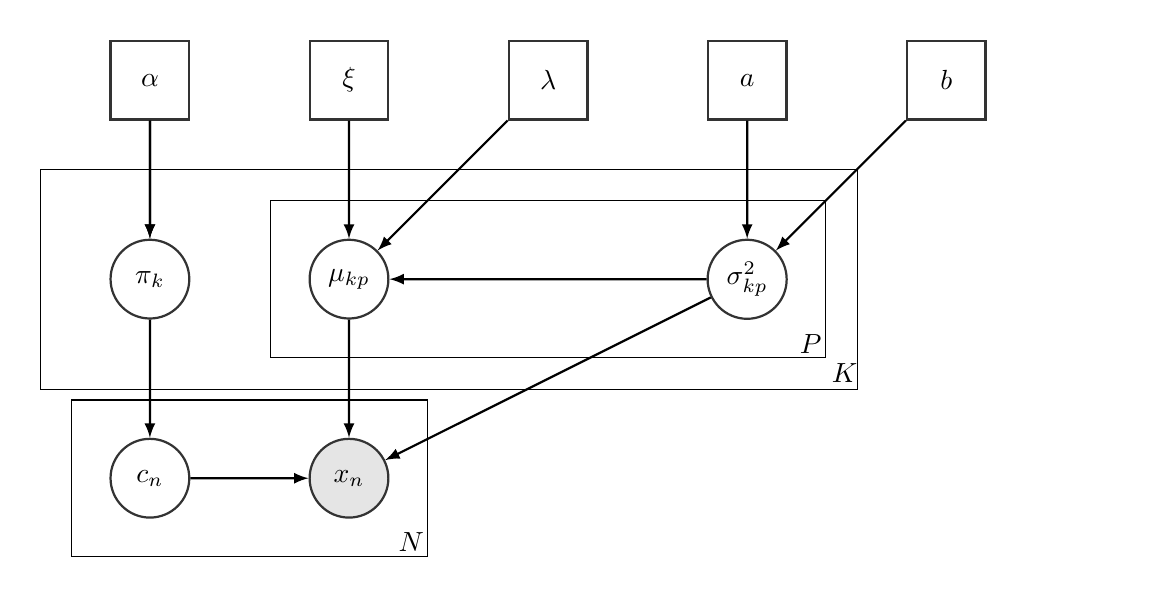
\begin{tikzpicture}[background rectangle/.style={fill=white!1}, show background rectangle, scale=.4, auto,>=latex']
		\tikzstyle{main}=[circle, minimum size = 10mm, thick, draw =black!80, node distance = 15mm]
		\tikzstyle{connect}=[-latex, thick]
		\tikzstyle{box}=[rectangle, draw=black!100]
		%\node[main] (k) {$K$ };
		\node[main, rectangle] (kappa) {$\lambda$};
		\node[main, rectangle] (xi) [left =of kappa] {$\xi$ };
		\node[main, rectangle] (alpha) [left =of xi] {$\alpha$ };
		%		\node[main] (k) [above =of alpha] {$K$};
		\node[main, rectangle] (alpha2) [right =of kappa] {$a$ };
		\node[main, rectangle] (beta) [right =of alpha2] {$b$ };
		\node[main] (pi) [below =of alpha] {$\pi_k$ };
		\node[main] (c_i) [below =of pi] {$c_n$};
		\node[main] (mu) [below=of xi] {$\mu_{kp}$};		
		\node[main] (sigma) [below =of alpha2] {$\sigma^2_{kp}$};
		\node[main, fill = black!10] (x_i) [below =of mu] {$x_n$};
		\node[rectangle, inner sep=-0.5mm, fit= (c_i) (x_i),label=below right:$N$, xshift=13mm, yshift=-1mm] {};
		\node[rectangle, inner sep=4.8mm,draw=black!100, fit= (c_i) (x_i)] {};
		\node[rectangle, inner sep=-0.8mm, fit= (mu) (pi) (sigma),label=below right:$K$, xshift=43mm, yshift=-5mm] {};
		\node[rectangle, inner sep=8.8mm, draw=black! 100, fit= (mu) (pi) (sigma)] {};
		\node[rectangle, inner sep=-0.5mm, fit= (mu) (sigma),label=below right:$P$, xshift=26mm, yshift=-1mm] {};
		\node[rectangle, inner sep=4.8mm, draw=black! 100, fit= (mu) (sigma)] {};
		\path 
		%		(k) edge [connect, bend right=30] (pi)
		%		(k) edge [connect, bend left=30] (c_i)
		%(k) edge [connect, bend left=30] (mu)
		%(k) edge [connect] (sigma)
		(alpha) edge [connect] (pi)
		(pi) edge [connect] (c_i)
		(alpha) edge [connect] (pi)
		(c_i) edge [connect] (x_i)
		(mu) edge [connect] (x_i)
		(sigma) edge [connect] (x_i)
		(sigma) edge [connect] (mu)
		(xi) edge [connect] (mu)
		(kappa) edge [connect] (mu)
		(alpha2) edge [connect] (sigma)
		(beta) edge [connect] (sigma)
		%(k) edge[connect, bend right=30] (x_i)
		;
	\end{tikzpicture}
	\caption{Directed acyclic graph for the mixture of Gaussians used.}
	\label{fig:simpleMixNormalsDAG}
\end{figure}

\subsection{Integrative clustering}
We are interested in the use of Consensus clustering for integrative methods. We use Multiple Dataset Integration \citep[\textbf{MDI}, ][]{kirk2012bayesian} as an example of a Bayesian integrative clustering method. 

%We use the implementation made by \citep{mason2016mdi} which produces MCMC samples of the allocation vector and is thus suited to our construction of Consensus clustering.

%Bayesian mixture models have been extended to the multiple dataset context where they are used to perform integrative clustering. This means that as much pertinent information as possible can be included in the joint model. Multiple Dataset Integration \citep[\textbf{MDI}, ][]{kirk2012bayesian} is an example of such a model where dataset specific clusterings are learnt, informed by common information. We use MDI to model the clustering structure of the Yeast datasets in section \ref{sec:yeast}. The modelling of the shared information is described by the prior distribution on item allocation for $L$ datasets

In MDI information is shared between datasets. Dataset specific clusterings are modelled with more information shared between datasets with more similar clustering structure. This can be seen in the prior on the allocation of the $n^{th}$ item across $L$ datasets
\begin{align}
	p(c_{n1}, \ldots, c_{nL}) \propto \prod_{l=1}^L \pi_{c_{nl}l}\prod_{l=1}^{L-1}\prod_{m=l+1}^L(1 + \phi_{lm} \mathbb{I}(c_{nl} = c_{nm})) \textrm{ for $n = 1,\ldots,N$.}
	\label{eqn:mdiPrior}
\end{align}
$\phi_{lm}$ is the parameter defined by the correlation of the clusterings for the $l^{th}$ and $m^{th}$ datasets and is also sampled in each iteration. As $\phi_{lm}$ increases more mass is placed on the common partition for these datasets. Conversely, in the limit $\phi_{lm}\to 0$ we have independent mixture models. The DAG for this model for three datasets is shown in figure \ref{fig:MDIDAG}.
\begin{sidewaysfigure}
	\centering
	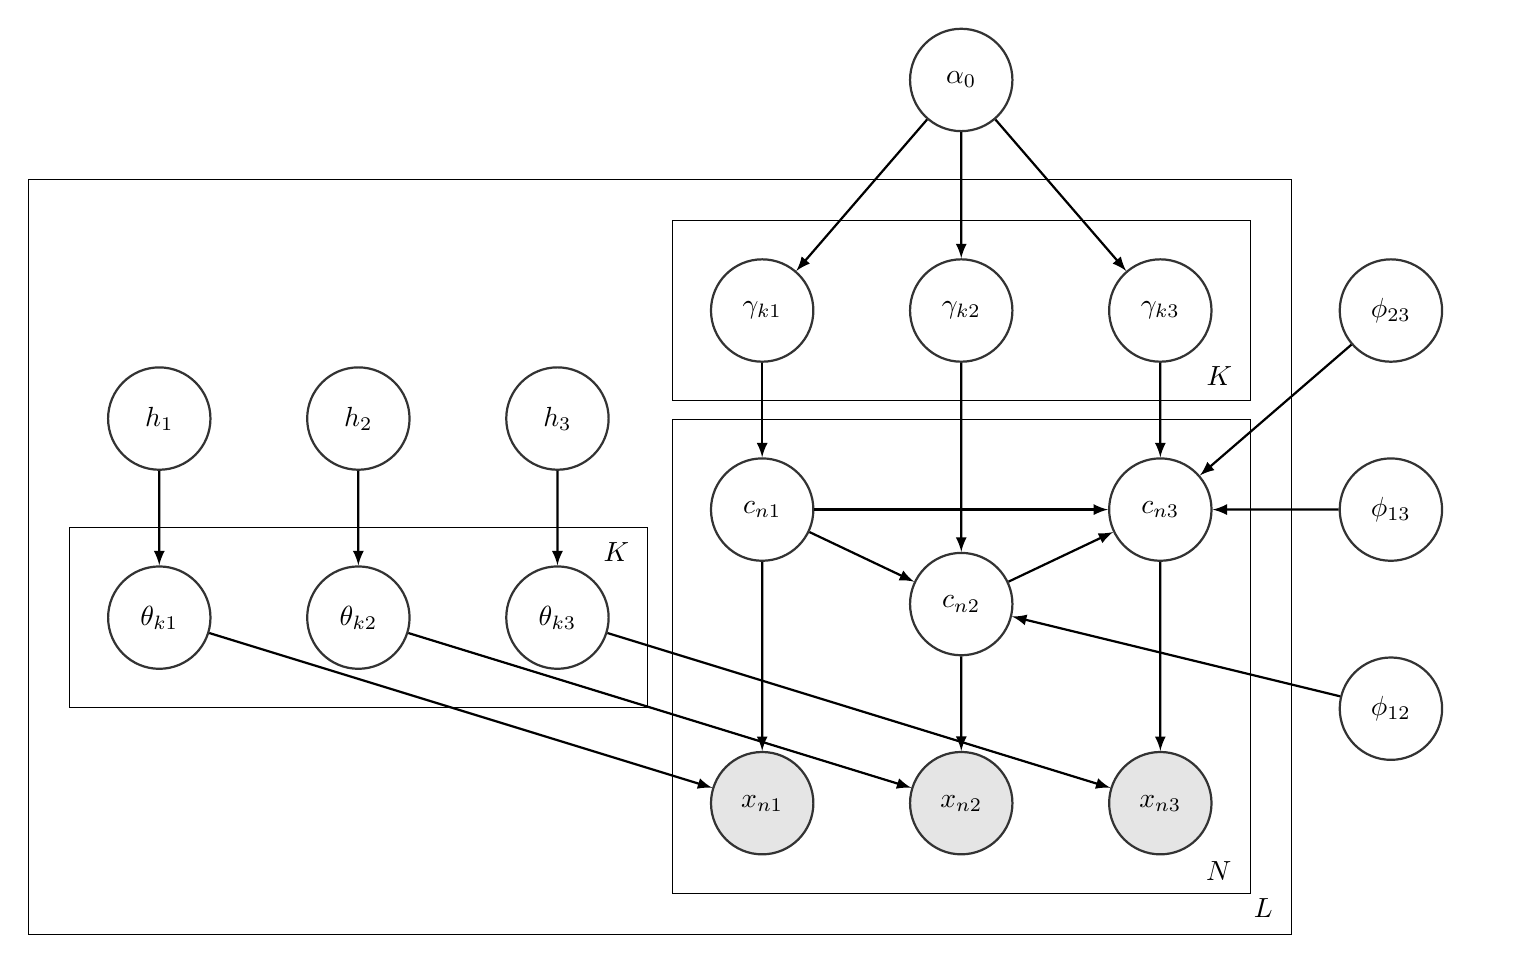
\begin{tikzpicture}[scale=.65, auto,>=latex']
	\tikzstyle{main}=[circle, minimum size = 13mm, thick, draw =black!80, node distance = 12mm]
	\tikzstyle{connect}=[-latex, thick]
	\tikzstyle{box}=[rectangle, draw=black!100]
	
	\node[main] (pi1) {$\gamma_{k1}$ };
	\node[main] (pi2) [right=of pi1] {$\gamma_{k2}$ };
	\node[main] (pi3) [right=of pi2] {$\gamma_{k3}$ };
	
	\node[main] (ci1) [below=of pi1] {$c_{n1}$};
	\node[main, node distance = 24mm] (ci2) [below=of pi2] {$c_{n2}$};
	\node[main] (ci3) [below=of pi3] {$c_{n3}$};
	
	\node[main, node distance = 16mm] (a) [above=of pi2] {$\alpha_0$ };
	
	\node[main, fill = black!10] (xi2) [below=of ci2] {$x_{n2}$}; 
	\node[main, fill = black!10] (xi1) [left=of xi2] {$x_{n1}$};
	\node[main, fill = black!10] (xi3) [right=of xi2] {$x_{n3}$};
	
	\node[main]  at (-4, -6) (theta3) {$\theta_{k3}$}; 
	\node[main] (theta2) [left=of theta3] {$\theta_{k2}$};
	\node[main] (theta1) [left=of theta2] {$\theta_{k1}$};
	
	
	\node[main] (h1) [above=of theta1] {$h_1$};
	\node[main] (h2) [above=of theta2] {$h_2$};
	\node[main] (h3) [above=of theta3] {$h_3$};
	
	\node[main, minimum size=1.3cm, node distance = 16mm] (phi13) [right=of ci3] {$\phi_{13}$}; 
	\node[main, minimum size=1.3cm] (phi12) [below=of phi13] {$\phi_{12}$};
	\node[main, minimum size=1.3cm] (phi23) [above=of phi13] {$\phi_{23}$};
	
	\node[rectangle, inner sep=-0.5mm, fit= (ci1) (ci2) (ci3) (xi1) (xi2) (xi3),label=below right:$N$, xshift=5mm, yshift=0mm] {};
	\node[rectangle, inner sep=4.8mm,draw=black!100, fit= (ci1) (ci2) (ci3) (xi1) (xi2) (xi3)] {};
	
	% \node[rectangle, inner sep=-0.8mm, fit= (theta1) (theta2) (theta3) (pi1) (pi2) (pi3) ,label=above right:$K$, xshift=63mm] {};
	% \node[rectangle, inner sep=4.8mm, draw=black! 100, fit= (theta1) (theta2) (theta3) (pi1) (pi2) (pi3)] {};
	
	\node[rectangle, inner sep=-0.8mm, fit= (theta1) (theta2) (theta3) ,label=above right:$K$, xshift=24mm] {};
	\node[rectangle, inner sep=4.8mm, draw=black! 100, fit= (theta1) (theta2) (theta3)] {};
	
	\node[rectangle, inner sep=-0.8mm, fit=  (pi1) (pi2) (pi3) ,label=below right:$K$, xshift=24mm] {};
	\node[rectangle, inner sep=4.8mm, draw=black! 100, fit= (pi1) (pi2) (pi3)] {};
	
	\node[rectangle, inner sep=-0.8mm, fit= (ci1) (ci2) (ci3) (xi1) (xi2) (xi3) (theta1) (theta2) (theta3) (pi1) (pi2) (pi3) (h1) (h2) (h3),label=below right:$L$, xshift=37mm, yshift=-5mm] {};
	\node[rectangle, inner sep=10.0mm, draw=black! 100, fit= (ci1) (ci2) (ci3) (xi1) (xi2) (xi3) (theta1) (theta2) (theta3) (pi1) (pi2) (pi3) (h1) (h2) (h3)] {};
	
	\path (pi1) edge [connect] (ci1)
	(pi2) edge [connect] (ci2)
	(pi3) edge [connect] (ci3)
	
	(ci1) edge [connect] (xi1)
	(ci2) edge [connect] (xi2)
	(ci3) edge [connect] (xi3)
	
	(ci1) edge [connect] (ci2)
	(ci1) edge [connect] (ci3)
	(ci2) edge [connect] (ci3)
	
	(theta1) edge [connect] (xi1)
	(theta2) edge [connect] (xi2)
	(theta3) edge [connect] (xi3)
	
	(h1) edge [connect] (theta1)
	(h2) edge [connect] (theta2)
	(h3) edge [connect] (theta3)
	
	(a) edge [connect] (pi1)
	(a) edge [connect] (pi2)
	(a) edge [connect] (pi3)
	
	(phi12) edge [connect] (ci2)
	(phi13) edge [connect] (ci3)
	(phi23) edge [connect] (ci3);
	
\end{tikzpicture}
	\caption{Directed acyclic graph for the Multiple Dataset Integration model for $L=3$ datasets.}
	\label{fig:MDIDAG}
\end{sidewaysfigure}
\section{Simulations} \label{sec:simulations}
A number of scenarios are defined by the parameters that they use in generating individual simulations using algorithm \ref{algorithm:simulationGeneration}. These parameters are shown in table \ref{table:scenarioTable}.
\begin{table}[ht]
	\centering
	% To place a caption above a table
%	\caption{Caption above table.}
	\begin{tabular}{|l|ccccccc|}
	\hline
	\textbf{Scenario} & $N$ & $P_s$ & $P_n$ & $K$ & $\Delta\mu$ & $\sigma^2$ & $\pi$\\
	\hline 
	2D & 100 & 2 & 0 & 5 & 3.0 & 1 &  $(\frac{1}{5} , \frac{1}{5}, \frac{1}{5}, \frac{1}{5}, \frac{1}{5})$ \\
	%		\hline
	No structure & 100 & 0 & 2 & 1 & 0.0 & 1 & 1 \\
	%		\hline
	Base Case & 200 & 20 & 0 & 5 & 1.0 & 1 &  $(\frac{1}{5} , \frac{1}{5}, \frac{1}{5}, \frac{1}{5}, \frac{1}{5})$\\
	%		\hline
	Large standard deviation & 200 & 20 & 0 & 5 & 1.0 & 9 & $(\frac{1}{5} , \frac{1}{5}, \frac{1}{5}, \frac{1}{5}, \frac{1}{5})$ \\
	%		\hline
	Large standard deviation & 200 & 20 & 0 & 5 & 1.0 & 25 &  $(\frac{1}{5} , \frac{1}{5}, \frac{1}{5}, \frac{1}{5}, \frac{1}{5})$\\
	%		\hline
	Irrelevant features & 200 & 20 & 10 & 5 & 1.0 & 1 &  $(\frac{1}{5} , \frac{1}{5}, \frac{1}{5}, \frac{1}{5}, \frac{1}{5})$\\
	%		\hline
	Irrelevant features & 200 & 20 & 20 & 5 & 1.0 & 1 &  $(\frac{1}{5} , \frac{1}{5}, \frac{1}{5}, \frac{1}{5}, \frac{1}{5})$\\
	%		\hline
	Irrelevant features & 200 & 20 & 100 & 5 & 1.0 & 1 &  $(\frac{1}{5} , \frac{1}{5}, \frac{1}{5}, \frac{1}{5}, \frac{1}{5})$\\
	%		\hline
	Varying proportions & 200 & 20 & 0 & 5 & 1.0 & 1 & $(\frac{1}{2} , \frac{1}{4}, \frac{1}{8}, \frac{1}{16}, \frac{1}{16})$ \\
	Varying proportions & 200 & 20 & 0 & 5 & 0.4 & 1 &  $(\frac{1}{2} , \frac{1}{4}, \frac{1}{8}, \frac{1}{16}, \frac{1}{16})$ \\ %(0.5, 0.25, 0.125, 0.0675, 0.0675)\\
	%		\hline
	Small N, large P & 50 & 500 & 0 & 5 & 1.0 & 1 &  $(\frac{1}{5} , \frac{1}{5}, \frac{1}{5}, \frac{1}{5}, \frac{1}{5})$\\
	%		\hline
	Small N, large P & 50 & 500 & 0 & 5 & 0.2 & 1 &  $(\frac{1}{5} , \frac{1}{5}, \frac{1}{5}, \frac{1}{5}, \frac{1}{5})$
	\\
	\hline
	\end{tabular}
	\caption{Parameters defining the simulation scenarios as used in generating data and labels.}
	\label{table:scenarioTable}
\end{table}%
\begin{algorithm} \label{algorithm:simulationGeneration}
	\TitleOfAlgo{Simulation generation}
	%	\KwData{\(X=(x_1, \ldots, x_N)\)}
	\KwIn{
		%		A random seed $s$\\
		Distance between means \(\Delta_{\mu}\)\\
		A common standard deviation \(\sigma^2\)\\
		A number of clusters \(K\)\\
		The number of items to generate in total \(N\)\\
		The number of features to generate in total \(P\)\\
		An indicator vector of feature relevance \(\phi = (\phi_1, \ldots, \phi_P)\)\\
		The expected proportion of items in each cluster \(\pi=(\pi_1, \ldots, \pi_K)\)\\
		A method for sampling \(x\) times from the array \(y\), with weights \(\pi\): \emph{Sample}\((y, x, \pi)\)\\
		A method for permuting a vector \(x\): \emph{Permute}\((x)\)\\
		A method for generating a value from a univariate Gaussian distribution with mean \(\mu\) and standard deviation \(\sigma^2\): \emph{Gaussian}\((\mu, \sigma^2)\)\\
	}
	\KwOut{A dataset, $X$ \\ The generating cluster labels $c=(c_1, \ldots, c_N)$}
	%	\KwResult{how to write algorithm with \LaTeX2e }
	\Begin{
		%		\tcc{Set the random seed defining the sampling and permuting}
		%		$set.seed(s)$\;
		\tcc{initialise the empty data matrix}
		$X \leftarrow 0_{N \times P}$\;
		\tcc{create a matrix of \(K\) means}
		$\mu \leftarrow (\Delta_{\mu}, \ldots, K\Delta_{\mu})$\;
		\tcc{generate the allocation vector}
		\(c \leftarrow\) \emph{Sample}\((1:K, N, \pi)\)\;
		
		$\mathbf{M} \leftarrow \mathbf{0}_{N \times N}$\;
		\For{$p = 1$ \KwTo $P$}{
			\tcc{Test if the feature is relevant, if relevant generate data from a mixture of univariate Gaussians, otherwise draw all items from the same distribution}
			\If{$\phi_p = 1$}{
				
				%				\tcc{Permute the means associated with each cluster within the current feature to create independent features}
				$\nu \leftarrow$ \emph{Permute}$(\mu)$\;
				
				\For{$n = 1$ \KwTo $N$}{
					%					\tcc{Generate data defined by the original label}
					\(X(n, p) \leftarrow\) \emph{Gaussian}\((\nu_{c_n}, \sigma^2)\)
				}
			}
			\If{$\phi_p = 0$}{
				\For{$n = 1$ \KwTo $N$}{
					\(X(n, p) \leftarrow\) \emph{Gaussian}\((0, \sigma^2)\)
				}
			}
		}
		\tcc{Mean centre and scale the data}
		$X \leftarrow Normalise(X)$
	}
	\caption{Data generation for a mixture of Gaussian with independent features. This algorithm is implemented in the \texttt{generateSimulationDataset} function from the \texttt{mdiHelpR} package available at \texttt{www.github.com/stcolema/mdiHelpR}.}
\end{algorithm}
We included each scenario to test certain concepts of the method and to explore behaviour due to specific characteristics of real data.
\begin{itemize}
	\item \emph{2D}: a low dimensional scenario within which we expect \texttt{Mclust} to perform well and the long chains to converge and explore the full support of the posterior distribution.
	\item \emph{No structure}: included to reassure fears that Consensus clustering has a predilection to finding clusters where none exist \citep{senbabaoglu2014reassessment,senbabaouglu2014critical}.
	\item \emph{Base case}: highly informative datasets that all methods are expect to find the true generating labels quite easily and is included to benchmark other scenarios that are variations of this setting.
	\item \emph{Large standard deviation}: these two scenarios investigate the degree of distinction required between clusters for the methods to uncover their structure.
	\item \emph{Irrelevant features}: these scenarios investigate how robust the methods are to irrelevant features.
	\item \emph{Varying proportions}: these scenarios investigate how well each method uncovers clusters when the clusters have significantly different membership counts.
	\item \emph{Small $N$, large $P$}: an investigation of behaviour when the number of features is far greater than the number of items.
\end{itemize}

\subsection{Bayesian analysis} \label{sec:simBayesianAnalysis}
For each simulation we run 10 chains of 1 million iterations. These chains are then thinned to every thousandth sample. We used discarded the first 10,000 iterations to remove burn-in bias. This leaves 990 samples per chain. To check if the chains were converged we used
\begin{itemize}
	\item the Geweke convergence diagnostic \citep{geweke1991evaluating} to investigate within-chain stationarity, and
	\item the potential scale reduction factor \citep[$\hat{R}$, ][]{gelman1992inference} and the Vats-Knudson extension \citep[\emph{stable $\hat{R}$},][]{vats2018revisiting} to check across-chain convergence.
\end{itemize}
The Geweke convergence diagnostic is a standard Z-score; it compares the sample mean of two sets of samples (in this case buckets of samples from the first half of the samples to the sample mean of the entire second half of samples). It is calculated under the assumption that the two parts of the chain are asymptotically independent and if this assumption holds (i.e. the chain is sampling the same distribution in both samples) than the scores are expected to be standard normally distributed. If a chain's Geweke convergence diagnostic passed a Shapiro-Wilks test for normality \citep{shapiro1965analysis} (based upon a threshold of 0.05), we considered it to have achieved stationarity and included it in the model performance analysis. 

$\hat{R}$ is expected to approach 1.0 if the set of chains are converged. Low $\hat{R}$ is not sufficient in itself to claim chain convergence, but values above 1.1 are clear evidence for a lack of convergence \citep{gelman2013bayesian}. \cite{vats2018revisiting} show that this threshold is significantly too high (1.01 being a better choice) and propose extensions to $\hat{R}$ that enable a more formal rule for a threshold. We use their method as implemented in the R package \texttt{stableGR} \citep{knudson20202stableGR} as the final check of convergence. An example of the $\hat{R}$ series across the 100 simulations for a scenario where chains are well-behaved is shown in figure \ref{fig:simBaseCaseRhat}.

\begin{figure} %[!tpb]
	\centering
	\includegraphics[scale=0.65]{./Images/Simulations/Convergence/base_caseConvergenceAcrossChains.png}
	\caption{The $\hat{R}$ values for each simulation (in dotted grey), the median value and the interquartile range. One can see that $\hat{R}$ approaches 1.0. The ``0\% of simulations failed to converge" is a statement based upon the percentage of simulations which passed the test of stable $\hat{R}$.}
	\label{fig:simBaseCaseRhat}
\end{figure}

We focus upon stationarity of the continuous variables. This is as assesing convergence of the allocation labels is difficult due to the label-switching problem. In our simulations, the only recorded continuous variable is the concentration parameter of the Dirichlet distribution for the component weights. 

We pooled the samples from the stationary chains and used these to form a Posterior similarity matrix. There are three possibilities to consider this decision under.
\begin{itemize}
	\item The chains are converged and agree upon the distribution sampled (see figure \ref{fig:simPSMsAgreeExample} for an example).
	\item The chains are not in agreement upon the partition sampled, becoming trapped in different modes. However, a mode does dominate being the mode present in a majority of chains (see figure \ref{fig:simPSMsDisagreeExample} for an example of this behaviour).
	\item The chains are not in agreement and no one mode dominates among chains.
\end{itemize}
In the first case pooling has no effect upon the predicted clustering compared to using any one chain. In the second case it feels natural that one would use the mode that dominates. Pooling the samples effectively does this for the predictive performance of the method as the mode with the greatest number of samples across the chains dominates, however the uncertainty for this mode is increased. In the third case the analysis is non-trivial and further thought, chains and samples would be required. Thankfully the generating process used means that only a small number of modes ever emerge in the PSMs and this case does not arise (based upon the simulations we investigated).

\begin{figure} %[!tpb]
	\centering
	\includegraphics[scale=0.65]{./Images/Simulations/PSMs/large_standard_deviation_3Sim1.png}
	\caption{Posterior similarity matrices for the simulation generated using a random seed set to 1 for the first large standard deviation scenario from table \ref{table:scenarioTable}. This is an example of all stationary chains agreeing in a simulation (and thus pooling of samples is no different to using any choice of chain for the performance analysis). Ordering of rows and columns is defined by hierarchical clustering of the first matrix in the series, in this case that from Chain 2.}
	\label{fig:simPSMsAgreeExample}
\end{figure}

\begin{figure} %[!tpb]
	\centering
	\includegraphics[scale=0.65]{./Images/Simulations/PSMs/small_n_large_p_baseSim1.png}
	\caption{Posterior similarity matrices for the simulation generated using a random seed set to 1 for the first small $N$, large $P$ scenario from table \ref{table:scenarioTable}. This is an example of different chains becoming trapped in different modes, but one mode (which does represent the generating structure well) is dominant, being fully present in 3 of the 6 chains, with the two other modes present having significant overlap. Ordering of rows and columns is defined by hierarchical clustering of the first matrix in the series, in this case that from Chain 3.}
	\label{fig:simPSMsDisagreeExample}
\end{figure}

\subsection{Consensus clustering analysis} 
A range of ensembles are investigated. All combinations of chain depth, $R=(1, 10, 100, 1000, 10000)$, and the number of chains, $S=(1, 10, 30, 50, 100)$ were used, a total of 25 different ensembles. A consensus matrix was constructed from the samples generated by each ensemble by finding the proportion of samples within which any pair of items are coclustered.

\subsection{\texttt{Mclust}}
\texttt{Mclust} was called using the default settings and a range of inputs for the choice of $K$. This was $K = (2, \ldots, \min(\frac{N}{2}, 50))$. The choice of $K=\min(\frac{N}{2}, 50)$ was made to mirror the default value of $K_{max}=50$ used for the overfitted mixture models, with the bound of $\frac{N}{2}$ to avoid fitting 50 clusters in the \emph{Small $N$, large $P$} scenario where $N=50=K_{max}$. The model choice is performed using the Bayesian Information Criterion \citep[][as implemented in \texttt{Mclust}]{schwarz1978estimating}.

% An example of each scenario may be seen in figure \ref{fig:genData}

\subsection{Model performance}
The different models (Bayesian (pooled), \texttt{Mclust} and the 25 Consensus clustering ensembles) were compared under their ability to predict the generating clustering and their uncertainty about this quantity.

\begin{sidewaysfigure} %[!tpb]
	\centering
	\includegraphics[scale=0.5]{./Images/Simulations/simulation_model_prediction.png}
	\caption{Predictive performance across all simulations. $CC(R, S)$ denotes consensus clustering using the $R^{th}$ sample from $S$ different chains.}
	\label{fig:simPrediction}
\end{sidewaysfigure}

\begin{sidewaysfigure} %[!tpb]
	\centering
	\includegraphics[scale=0.5]{./Images/Simulations/simulation_uncertainty.png}
	\caption{Frobenius norm across simulations. $CC(R, S)$ denotes consensus clustering using the $R^{th}$ sample from $S$ different chains. Lower values are better.}
	\label{fig:simUncertainty}
\end{sidewaysfigure}

\section{Yeast} \label{sec:yeast}

The "Yeast data" consists of three \emph{S. cerevisiae} datasets with gene products associated with a common set of 551 genes. The datasets are:
\begin{itemize}
	\item microarray profiles of RNA expression from \cite{granovskaia2010high}. This a cell cycle dataset that comprises measurements taken at 41 time points (the \textbf{Timecourse} dataset).
	\item Chromatin immunoprecipitation followed by microarray hybridization (\textbf{ChIP-chip}) data from \cite{harbison2004transcriptional}. This dataset has 117 features.
	\item Protein-protein interaction (\textbf{PPI}) data from BioGrid \citep{stark2006biogrid}. This dataset has 603 features.
\end{itemize}
The datasets were reduced to 551 items by considering only the genes identified by \cite{granovskaia2010high} as having periodic expression profiles with no missing data in the PPI and ChIP-chip data, following the same steps as the original MDI paper \citep{kirk2012bayesian}. The datasets were modelled using a base measure of a Gaussian process in the Timecourse dataset and Multinomial distributions in the ChIP-chip and PPI datasets.

\subsection{Bayesian analysis} \label{sec:yeastBayesianAnalysis}
We ran 10 chains of MDI for 36 hours saving every thousandth sample. This resulted in chains of varying length. We reduced the chains to 676 samples as this was the number of samples achieved by the slowest chain. Similar to section \ref{sec:simBayesianAnalysis} these chains were then investigated for 
\begin{itemize}
	\item within-chain stationarity using the Geweke convergence diagnostic \citep{geweke1991evaluating}, and
	\item across-chain convergence using $\hat{R}$ \citep{gelman1992inference} and the Vats-Knudson extension \citep[\emph{stable $\hat{R}$},][]{vats2018revisiting}.
\end{itemize}
%The Geweke convergence diagnostic is a standard Z-score; it compares the sample mean of two sets of samples (in this case buckets of samples from the first half of the samples to the sample mean of the entire second half of samples). It is calculated under the assumption that the two parts of the chain are asymptotically independent and if this assumption holds than the scores are expected to be standard normally distributed presenting evidence for within chain stationarity.
%
%$\hat{R}$ is expected to approach 1.0 if the set of chains are converged. Low $\hat{R}$ is not sufficient in itself to claim chain convergence, but values above 1.1 are clear evidence for a lack of convergence \citep{gelman2013bayesian}. \cite{vats2018revisiting} show that this threshold is significantly too high (1.01 being a better choice) and propose extensions to $\hat{R}$ that enable a more formal rule for a threshold. It is their method as implemented in the R package \texttt{stableGR} \citep{knudson20202stableGR} that is the final check of convergence.
%
Again we focus upon stationarity of the continuous variables. In the implementation of MDI we used \cite{mason2016mdi}, the recorded continuous variables are the concentration parameters of the Dirichlet distribution for the dataset-specific component weights and the $\phi_{ij}$ parameter associated with the correlation between the $i^{th}$ and $j^{th}$ datasets. 
\begin{figure}
	\centering
	\includegraphics[scale=1.0]{./Images/Yeast/Convergence/gewekePlot.png}
	\caption{Chain 9 can be seen to have the most extreme behaviour in the distribution of the Geweke diagnostic for the parameters. We remove this chain from the analysis. Of the remaining chains we believe that 1, 2, 4 and 6 express the distributions furthest removed from the desired behaviour and are dropped from the analysis.}
	\label{fig:gewekePlot}
\end{figure}

%\begin{figure}
%	\centering
%	\includegraphics[scale=0.7]{./Images/Yeast/Convergence/gewekePhiChain.png}
%	\caption{None of the chains appear to be standard normal in their distribution. Chain 4 behaves very strangely and is also dropped from the analysis. Of the remaining chains there is less clear distinctions, but chains 1, 2, and 6 appear most extreme and thus are dropped.}
%	\label{fig:gewekePhiPlot}
%\end{figure}
We plot the Geweke-statistic for each chain in figure \ref{fig:gewekePlot}. No chain is perfectly behaved; as we cannot reduce to the set of stationary chains we thus exclude the most poorly behaved chains. Our lack of belief in the convergence of these chains is fortified by the behaviour of $\hat{R}$ (which can be seen in figure \ref{fig:gelmanPlot}) and the different distributions sampled for the $\phi_{lm}$ parameters shown in figure \ref{fig:bayesDensities}.
%where the values of $\hat{R}$ do not drop below 1.25 for the $\phi$ parameters. Stable $\hat{R}$ is also too high, with several million more samples recommended before convergence is expected.
\begin{figure}
	\centering
	\includegraphics[scale=1.0]{./Images/Yeast/Convergence/gelmanPlot.png}
	\caption{The chains still appear to be unconverged with $\hat{R}$ remaining above 1.25 for the $\phi_{12}, \phi_{13}$ and $\phi_{23}$ parameters. Stable $\hat{R}$ is also too high with values of 1.049, 1.052 and 1.057.}
	\label{fig:gelmanPlot}
\end{figure}
\begin{figure}
	\centering
	\includegraphics[scale=1]{./Images/Yeast/densityPlotReduced.png}
	\caption{The densities of the continuous variables across the 5 chains kept for analysis. The mean sampled values are $\alpha_1= 64.84$, $\alpha_2 = 69.85$, $\alpha_2 = 63.22$, $\phi_{12} = 81.76$, $\phi_{13} = 13.87$, and $\phi_{23} = 65.03$. It can be seen that different modes are being sampled for the $\phi$ parameters in each chain.
	}
	\label{fig:bayesDensities}
\end{figure}

We visualise the the PSMs for each dataset in figure \ref{fig:yeastPSMs}. 
%The Timecourse data appears to have only the mildest of disagreement between the PSMs from different chains (see figure \ref{fig:timecoursePSMs}). The lack of convergence between chains emerges in the ChIP-chip data (figure \ref{fig:chipchipPSMs}) and, to a far greater degree, in the PPI data (figure \ref{fig:ppiPSMs}).

\begin{figure}
	\centering
	\includegraphics[scale=1.0]{./Images/Yeast/YeastPSMcomparisonReduced.png}
	\caption{PSMs for each chain within each dataset. The PSMs are ordered by hierarchical clustering of the rows of the PSM for chain 3 in each dataset. There is no marked difference between the matrices for the Timecourse data with disagreement becoming more prominent in the ChIP-chip data and more so again in the PPI dataset.}
	\label{fig:yeastPSMs}
\end{figure}


%\begin{figure}
%	\centering
%	\includegraphics[scale=0.5]{./Images/Yeast/TimecoursePSMcomparisonReduced.png}
%	\caption{The entries of each matrix are ordered by hierarchical clustering of the PSM for chain 3. There is no marked difference between matrices.}
%	\label{fig:timecoursePSMs}
%\end{figure}

%\begin{figure}
%	\centering
%	\includegraphics[scale=0.5]{./Images/Yeast/ChIP-chipPSMcomparisonReduced.png}
%	\caption{The entries of each matrix are ordered by hierarchical clustering of the PSM for chain 3. Disagreement can be seen between each chain.}
%	\label{fig:chipchipPSMs}
%\end{figure}

%\begin{figure}
%	\centering
%	\includegraphics[scale=0.5]{./Images/Yeast/PPIPSMcomparisonReduced.png}
%	\caption{The entries of each matrix are ordered by hierarchical clustering of the PSM for chain 3. These PSMs express very large disagreement about the clustering. There is some agreement with the square in the centre of each plot appearing similar in each PSM. However, the other sections (which consist of the most confident allocations) appear to completely fail to overlap.}
%	\label{fig:ppiPSMs}
%\end{figure}

\subsection{Consensus clustering analysis} \label{sec:consensusClustering}
We investigate an ensemble of depth $R=1001$ and width $S=10000$. The consensus matrices for this ensemble was compared to those for the combinations of $R = (1, 101, 501, 1001, 5001, 10001)$, $S=(1, 100, 500, 1,000)$ in the three datasets. We decide the ensemble is sufficiently deep and wide to stop growing if,  for a given depth $r$ and width $s$, there is no visible difference between the consensus matrices from the ensembles using $R=(a r, r)$, $S=(s, b s)$. In our analysis we used $a=b=0.5$ (the smaller the choice of $a,b$ the more extreme the stopping criterion). This heuristic is inspired by the belief that a clustering method should produce stable results across similar datasets \citep{von2005towards, meinshausen2010stability}. We believe that if the method is still producing a partition that is visibly changing for additional chains and depth, than the random initialisation is influencing the result sufficiently that it is unlikely to be stable for similar datasets or reproducible for a random choice of seeds (i.e. not stable within the current dataset). An example of this logic can be seen in figures \ref{fig:chipchipCMs} and \ref{fig:ppiCMs} (and to a lesser degree in figure \ref{fig:timecourseCMs}). Here the decision to stop growing the ensemble is made as there is no apparent gain in increasing chain depth from $R=5001$ to $R=10001$, but it can be seen that a chain depth of $R=1001$ is insufficient as there is a marked difference in the consensus matrices for the PPI dataset particularly between $R=1001$ and $R=5001$. The number of chains appears required appears to have stabilised quickly, as there is no obvious change in increasing $S$ from 100.

\begin{figure}
	\centering
	\includegraphics[scale=0.8]{./Images/Yeast/TimecourseCMcomparison.png}
	\caption{Consensus matrices for different ensembles of MDI for the Timecourse data. This dataset has stable clustering across the different choices of number of chains, $S$, and chain depth, $R$, with some components merging as the chain depth increases.}
	\label{fig:timecourseCMs}
\end{figure}

\begin{figure}
	\centering
	\includegraphics[scale=0.8]{./Images/Yeast/ChIP-chipCMcomparison.png}
	\caption{The ChIP-chip dataset is more sparse than the Timecourse data. In keeping with the results from the simulations for mixture models, deeper chains are required for better performance. It is only between $R=5,001$ and $R=10,001$ that no change in the clustering can be observed and the result is believed to be stable. In this dataset the number of chains used, $S$, appears relatively unimportant, with similar results for $S=100, 500, 1000$.}
	\label{fig:chipchipCMs}
\end{figure}

\begin{figure}
	\centering
	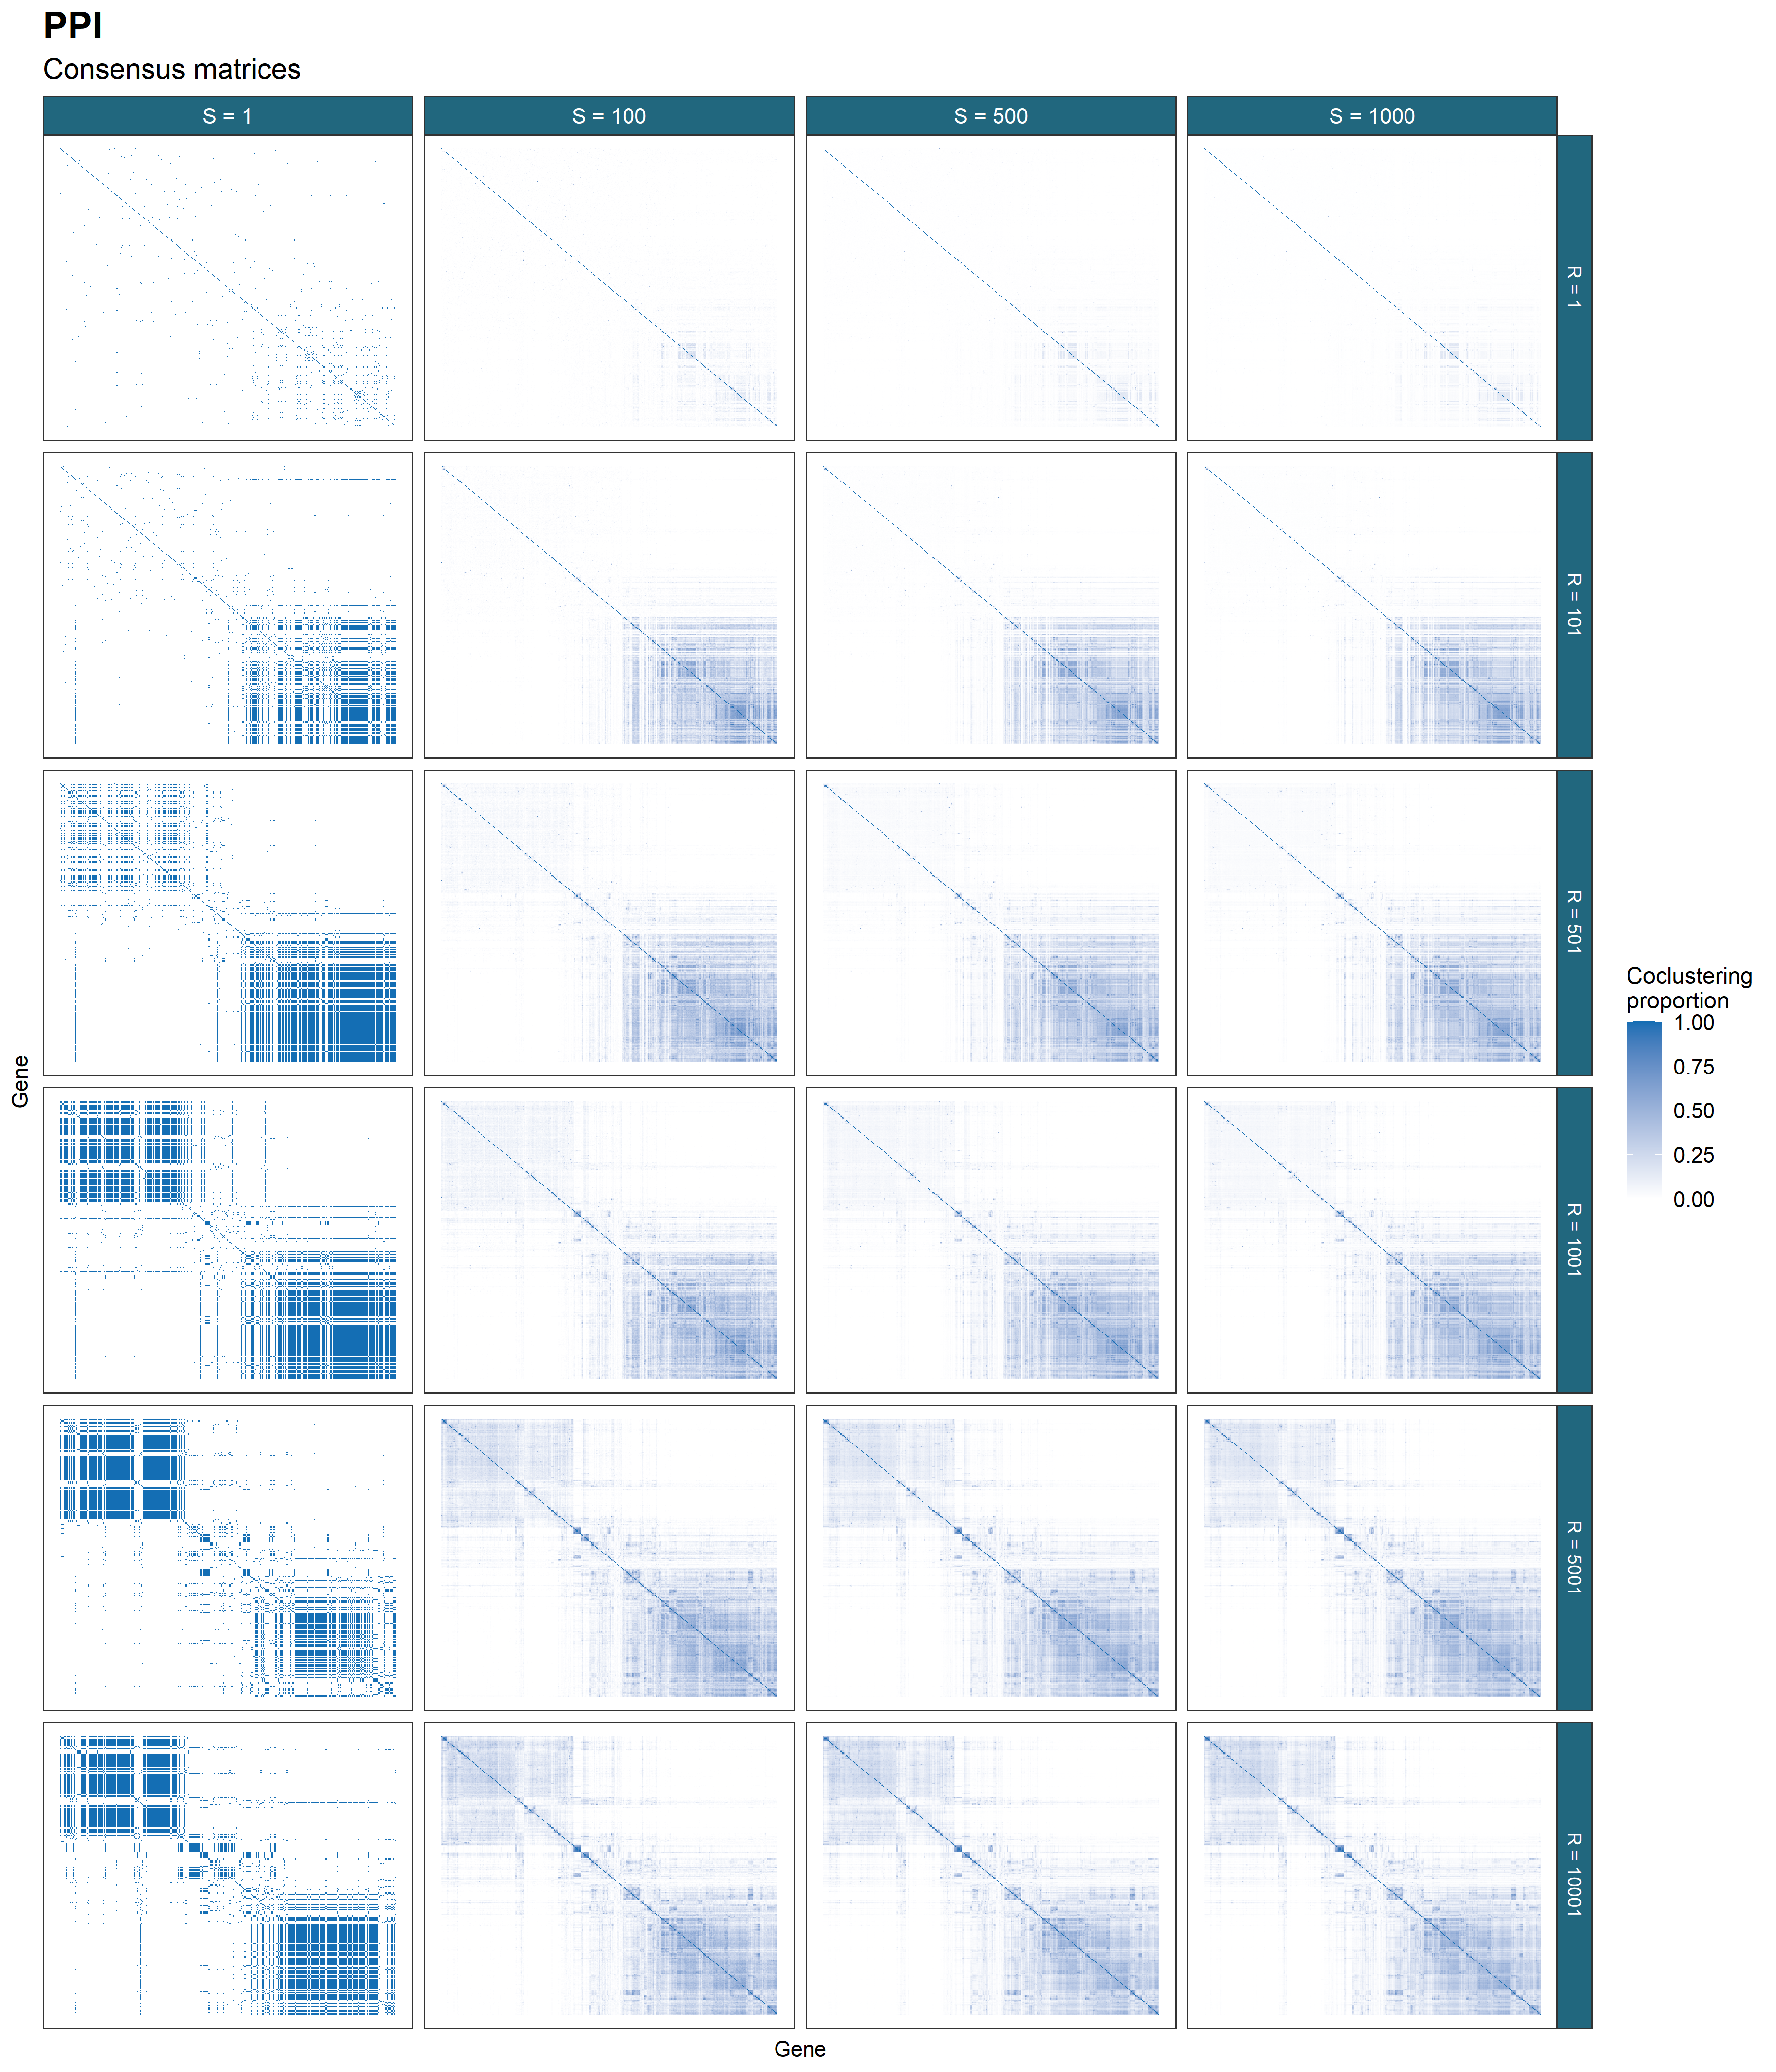
\includegraphics[scale=0.8]{./Images/Yeast/PPICMcomparison.png}
	\caption{The PPI dataset has awkward characteristics for modelling. A wide, sparse dataset it is again chain depth that is the most important parameter for the ensemble. Similar to the results in figure \ref{fig:chipchipCMs}, the matrices only stabilise from $R=5001$ to $R=10001$.}
	\label{fig:ppiCMs}
\end{figure}

If we compare the distribution of sampled values for the $\phi$ parameters for the Bayesian chains that we keep based upon their convergence diagnostics, the final ensemble used ($R=10001$, $S=1000$) and the pooled samples from the 5 long chains, then we see that the ensemble consisting of the long chains (which might be believed to sampling different parts of the posterior distribution) is closer in its appearance to the distributions sampled by the Consensus clustering than to any single chain.

\begin{figure}
	\centering
	\includegraphics[scale=0.6]{./Images/Yeast/ComparisonDensities.png}
	\caption{The sampled values for the $\phi$ parameters from the long chains, their pooled samples and the consensus using 1000 chains of depth 10,001. The long chains display a variety of behaviours. Across chains there is no clear consensus on the nature of the posterior distribution. The samples from any single chain are not particularly close to the behaviour of the pooled samples across all three parameters. It is the Consensus clustering that most approaches this pooled behaviour.}
	\label{fig:densityComparison}
\end{figure}

\subsection{GO term over-representation} \label{sec:goTermOverRep}
To validate the predicted clusters we test if they contain a higher concentration of specific Gene Ontology (GO) terms than would be expected by chance. Clusters were predicted from the PSMs of the chains kept from section \ref{sec:yeastBayesianAnalysis} visualised in figure \ref{fig:yeastPSMs} and the consensus matrix of the largest ensemble run (i.e. $CC(10001, 1000)$) using the \texttt{maxpear} function from the R package \texttt{mcclust} \cite{fritsch2012mcclust} using default settings except for \texttt{k.max} which was set to 275 (the rounding down of $N/2$). To perform the GO term over-representation analysis we used the \texttt{Bioconductor} packages \texttt{clusterProfiler} \citep{yu2012clusterProfiler}, \texttt{biomaRt} \citep{durinck2009mapping} and the annotation package \texttt{org.Sc.sgd.db} \citep{carlson2014org}.

We conditioned the test on the background set of the 551 yeast genes in the data. The gene labelled YIL167W was not found in the annotation database and was dropped from the analysis leaving a background universe of 550 genes. A hypergeometric test was used to check if the number of genes associated with specific GO terms within a cluster was greater than expected by random given the 550 possible genes. The false discovery rate of this test was controlled using the Benjamini-Hochberg correction \citep{benjamini1995controlling} and significance threshold of 0.05 was used. The over-represented GO terms were then plotted to compare methods. The three different ontologies of ``Molecular function" (\textbf{MF}), ``Biological process" (\textbf{BP}) and ``Cellular component" (\textbf{CC}) were all investigated. The over-represented terms are displayed in figures \ref{fig:yeastGOMF}, \ref{fig:yeastGOBP} and \ref{fig:yeastGOCC} respectively. It can be seen that the Consensus clustering finds very similar results to the long chains, finding any term that is over-represented in each chain and a number of terms unique to itself. Very few terms found by a single chain are over-represented in the clustering from the ensemble.

\begin{sidewaysfigure}
	\centering
	\includegraphics[scale=0.5]{./Images/Yeast/goEnrichmentCompMF.png}
	\caption{.}
	\label{fig:yeastGOMF}
\end{sidewaysfigure}

\begin{sidewaysfigure}
	\centering
	\includegraphics[scale=0.4]{./Images/Yeast/goEnrichmentCompBP.png}
	\caption{.}
	\label{fig:yeastGOBP}
\end{sidewaysfigure}

\begin{sidewaysfigure}
	\centering
	\includegraphics[scale=0.4]{./Images/Yeast/goEnrichmentCompCC.png}
	\caption{.}
	\label{fig:yeastGOCC}
\end{sidewaysfigure}

\bibliographystyle{plainnat}
\bibliography{suppMat}  

\end{document}
